\documentclass[compress]{beamer}
\usepackage{ifthen,verbatim}

\newcommand{\isnote}{}
\xdefinecolor{lightyellow}{rgb}{1.,1.,0.25}
\xdefinecolor{darkblue}{rgb}{0.1,0.1,0.7}
\xdefinecolor{darkgreen}{rgb}{0.1,0.7,0.1}

%% Uncomment this to get annotations
%% \def\notes{\addtocounter{page}{-1}
%%            \renewcommand{\isnote}{*}
%% 	   \beamertemplateshadingbackground{lightyellow}{white}
%%            \begin{frame}
%%            \frametitle{Notes for the previous page (page \insertpagenumber)}
%%            \itemize}
%% \def\endnotes{\enditemize
%% 	      \end{frame}
%%               \beamertemplateshadingbackground{white}{white}
%%               \renewcommand{\isnote}{}}

%% Uncomment this to not get annotations
\def\notes{\comment}
\def\endnotes{\endcomment}

\setbeamertemplate{navigation symbols}{}
\setbeamertemplate{headline}{\mbox{ } \hfill
\begin{minipage}{5.5 cm}
\vspace{-0.75 cm} \small
\end{minipage} \hfill
\begin{minipage}{4.5 cm}
\vspace{-0.75 cm} \small
\begin{flushright}
\ifthenelse{\equal{\insertpagenumber}{1}}{}{Jim Pivarski \hspace{0.2 cm} \insertpagenumber\isnote/\pageref{numpages}}
\end{flushright}
\end{minipage}\mbox{\hspace{0.2 cm}}\includegraphics[height=1 cm]{../cmslogo} \hspace{0.1 cm} \includegraphics[height=1 cm]{../tamulogo} \hspace{0.01 cm} \vspace{-1.05 cm}}

\begin{document}
\begin{frame}
\vfill
\begin{center}
\textcolor{darkblue}{\Large DT and CSC Alignments Proposed for \\ \vspace{0.25 cm} 2$^{\mbox{\scriptsize nd}}$ CRAFT-09 Reprocessing}

\vfill
\begin{columns}
\column{0.3\linewidth}
\begin{center}
\large
\textcolor{darkblue}{Jim Pivarski}
\end{center}
\end{columns}

\begin{columns}
\column{0.8\linewidth}
\begin{center}
\scriptsize
{\it On the behalf of the Muon Alignment Community}
\end{center}
\end{columns}

\vfill
4 November, 2009

\end{center}
\end{frame}

%% \begin{notes}
%% \item This is the annotated version of my talk.
%% \item If you want the version that I am presenting, download the one
%% labeled ``slides'' on Indico (or just ignore these yellow pages).
%% \item The annotated version is provided for extra detail and a written
%% record of comments that I intend to make orally.
%% \item Yellow notes refer to the content on the {\it previous} page.
%% \item All other slides are identical for the two versions.
%% \end{notes}

\small

\begin{frame}
\frametitle{Muon alignment preparation}

\textcolor{darkblue}{\Large \bf DT:} \hfill 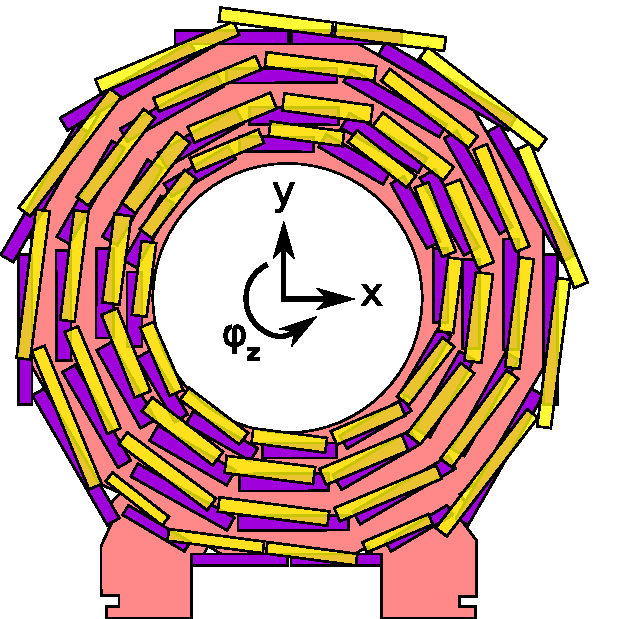
\includegraphics[height=2.3 cm]{global_dt.pdf} \hfill 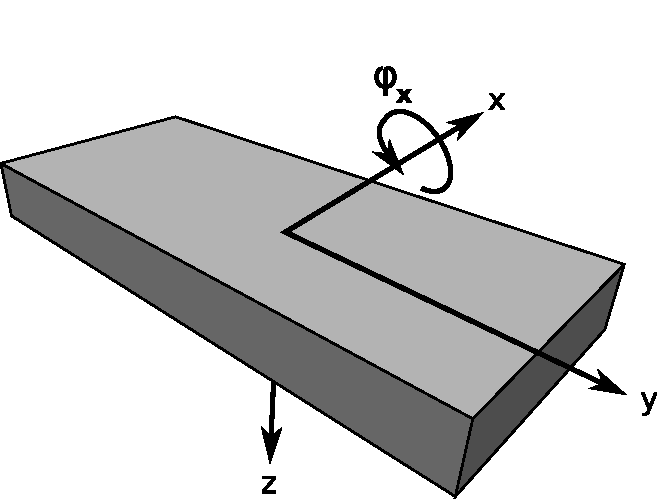
\includegraphics[height=2.3 cm]{dt_coordinates.pdf}

\begin{enumerate}
\item Hardware alignment system sets all coordinates
\item Position whole barrel as a rigid body in global $x$, $y$, $\phi_z$ with tracks
\item Align all accessible chambers, all parameters except $\phi_x$ with tracks
\end{enumerate}

\begin{columns}
\column{0.6\linewidth}
\textcolor{darkblue}{\Large \bf CSC:}
\begin{enumerate}
\item Hardware alignment sets $z$, \mbox{chamber $\phi_x$\hspace{-1 cm}}
\item Position whole rings as rigid bodies in global $x$, $y$, $\phi_z$ with tracks
\end{enumerate}

\column{0.3\linewidth}
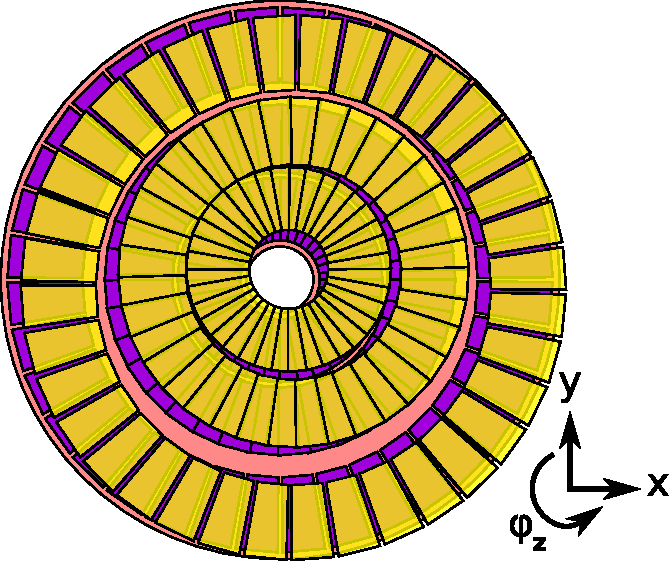
\includegraphics[height=2.3 cm]{global_csc.pdf}
\end{columns}

\vspace{0.5 cm}
\textcolor{darkblue}{\mbox{Any parameters unaligned by one step default to values from previous step\hspace{-1 cm}}}

\textcolor{darkblue}{\mbox{Final contributions are orthogonal, the best information each system provides\hspace{-1 cm}}}
\end{frame}

\begin{frame}
\frametitle{DT validation plots}
\begin{columns}
\column{0.6\linewidth}
\mbox{Repeated all checks developed in CRAFT-08:\hspace{-1 cm}}

\begin{itemize}
\item Fit functions overlaid on fitted distributions
\item ``Map plots'' (residuals versus position)
\item Distributions of medians of residuals
\item Local segment check: 0.35~mm for stations 1--3
\end{itemize}

\vfill
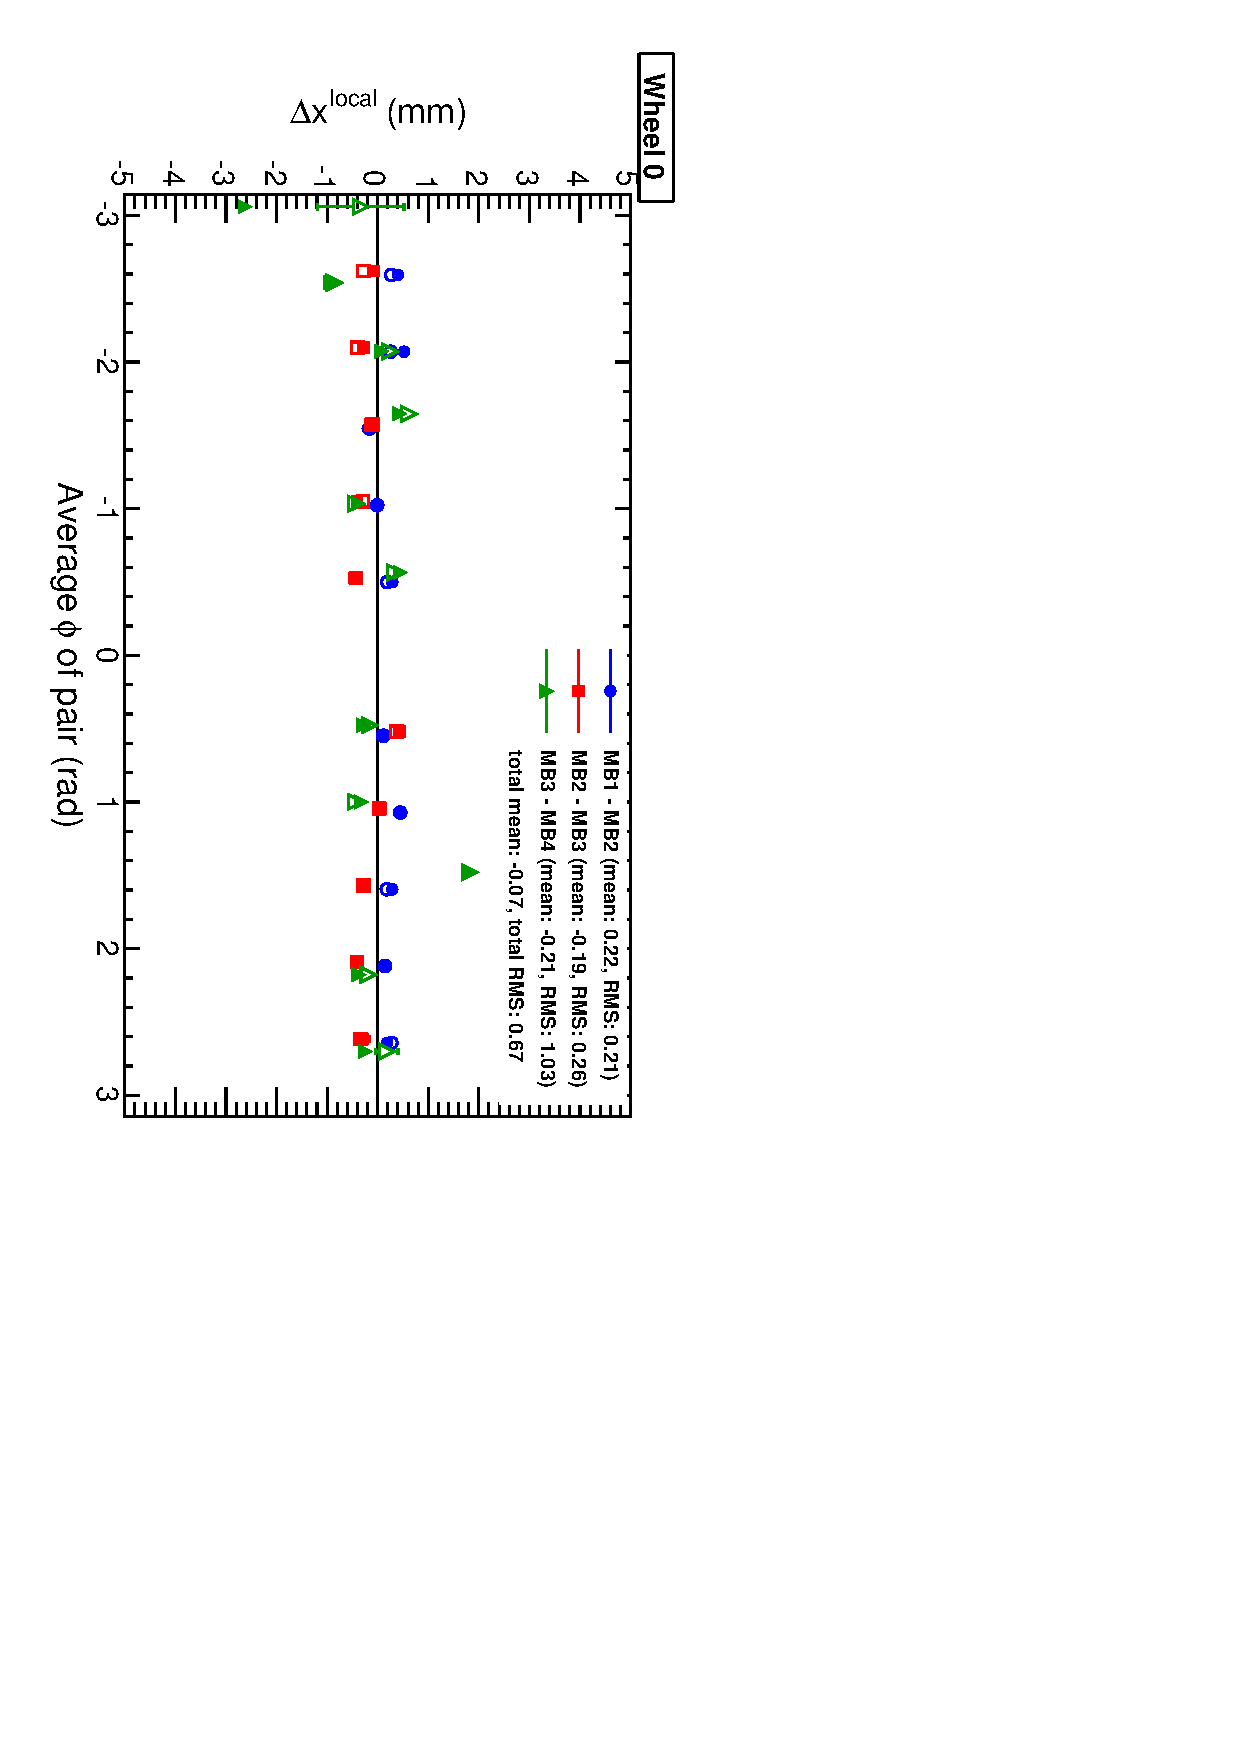
\includegraphics[height=\linewidth, angle=90]{NOV4_segdiff_x_whze.pdf}

\column{0.4\linewidth}
\vspace{-1 cm}
\hfill 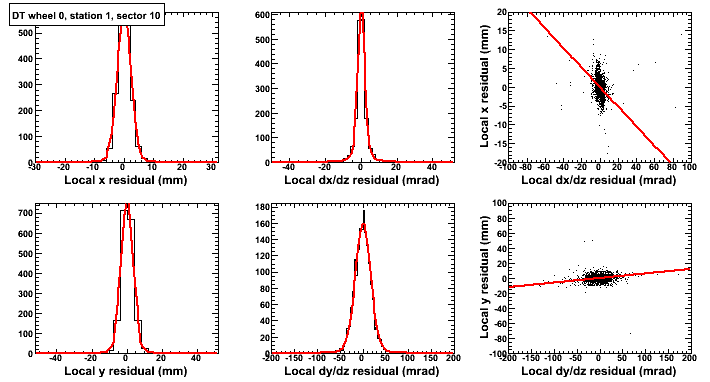
\includegraphics[width=0.8\linewidth]{NOV4_fitfunctions/MBwhCst1sec10_bellcurves.png}

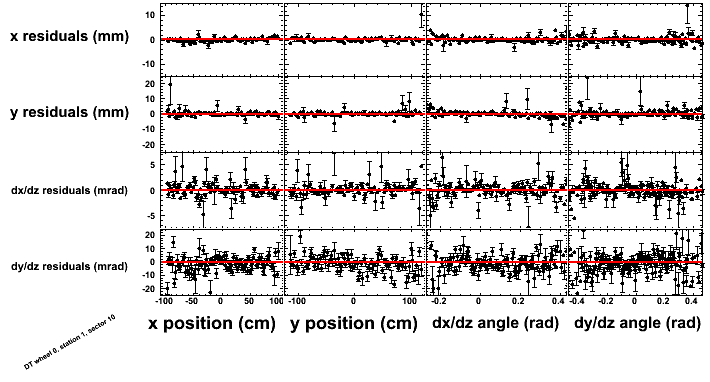
\includegraphics[width=\linewidth]{NOV4_fitfunctions/MBwhCst1sec10_polynomials.png}

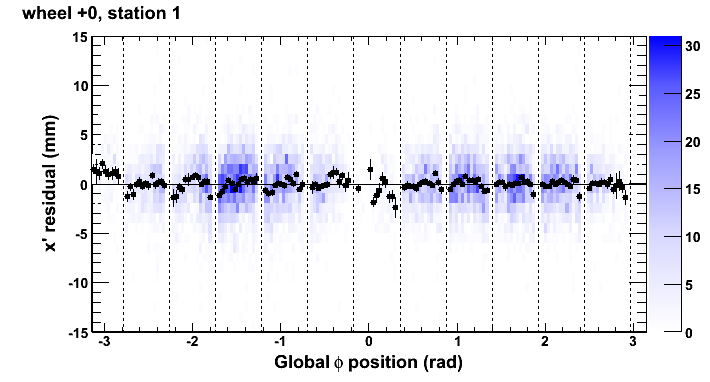
\includegraphics[width=\linewidth]{NOV4_mapplots/DTvsphi_st1whC_x.png}

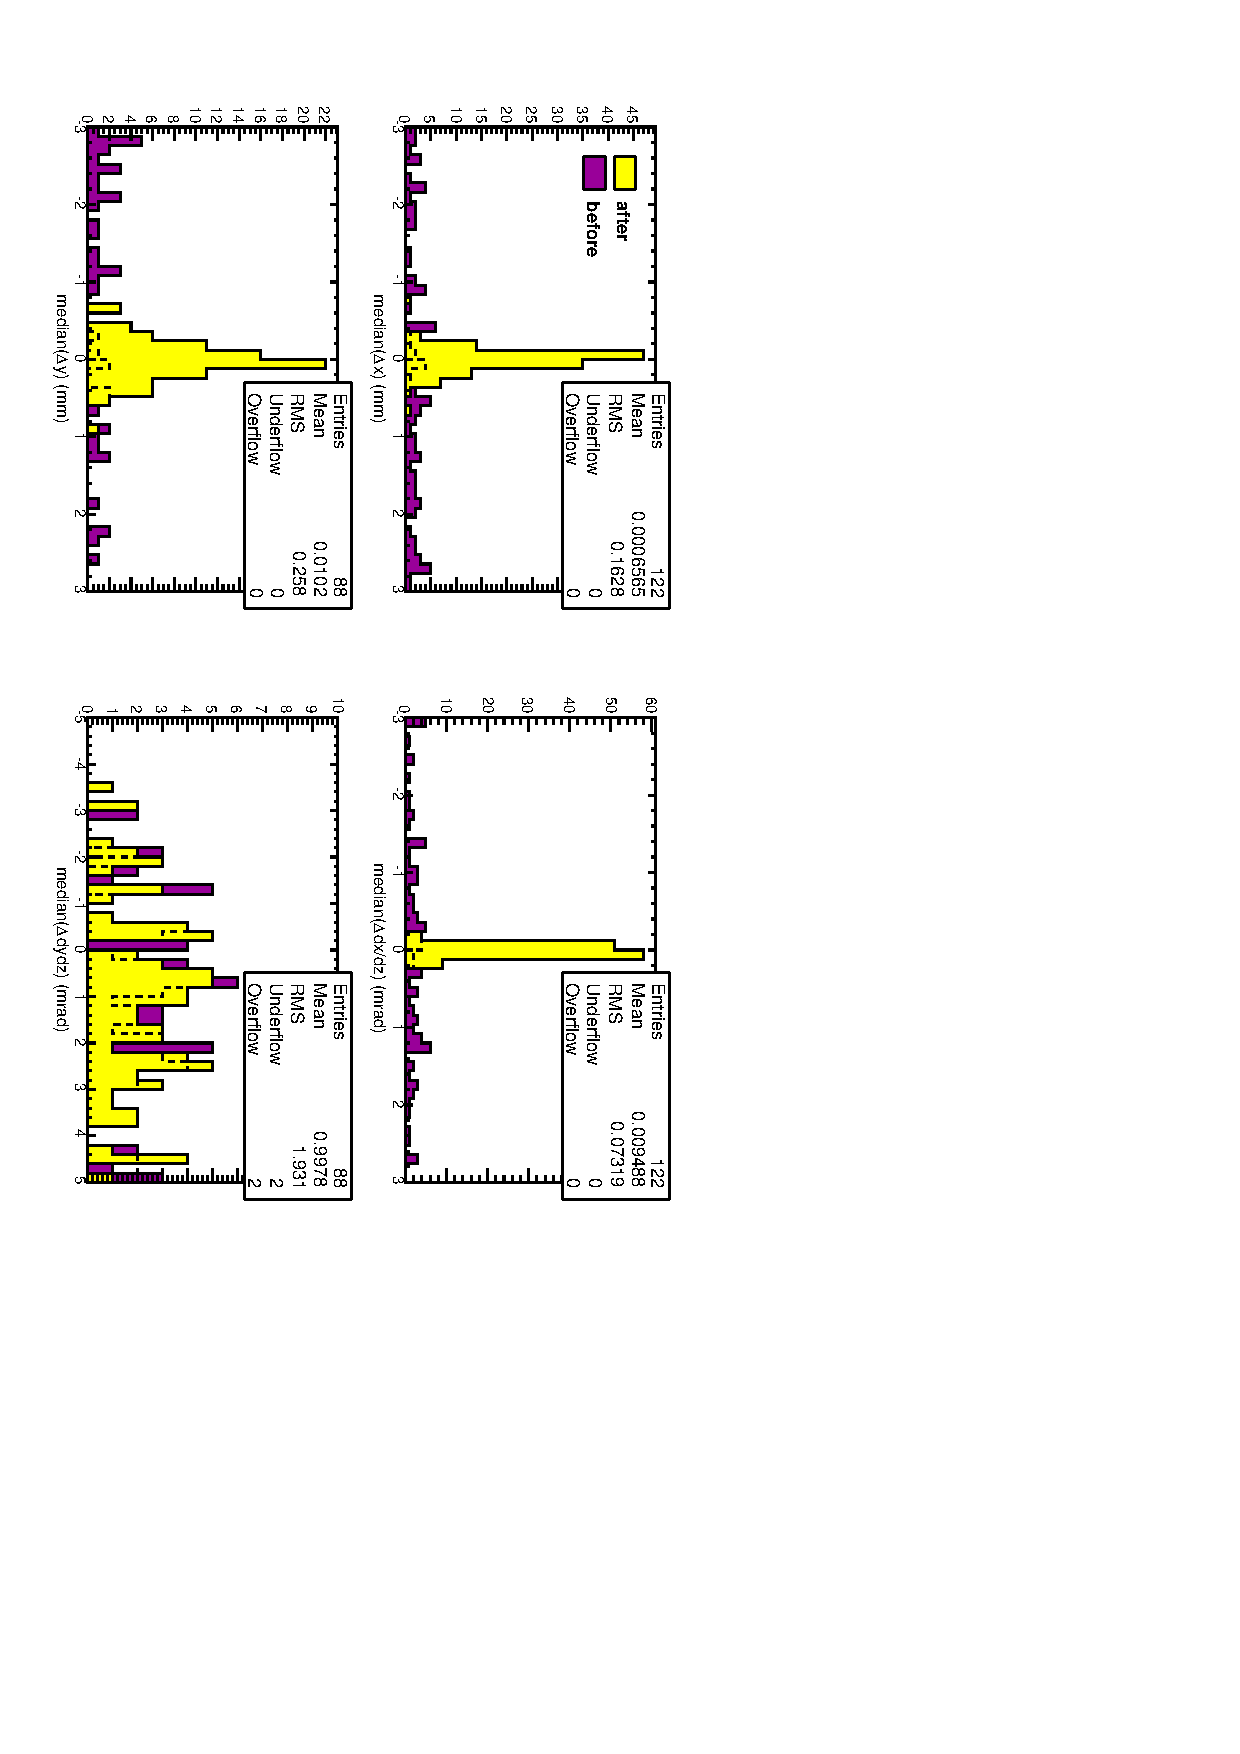
\includegraphics[height=\linewidth, angle=90]{NOV4DT_median_goodDT.pdf}
\end{columns}
\end{frame}

\begin{frame}
\frametitle{Cosmic splitting}
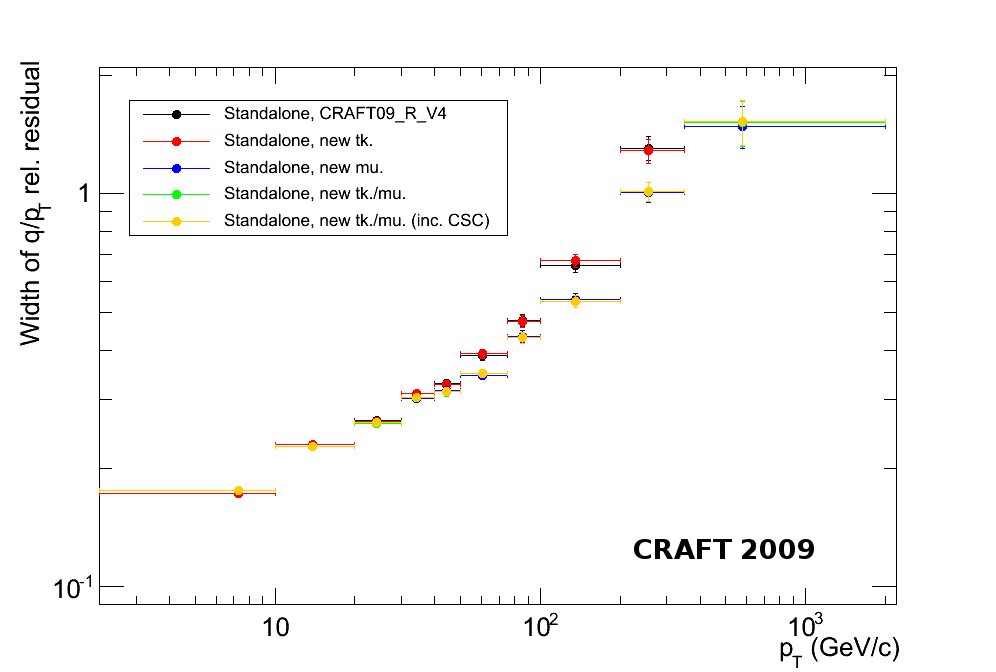
\includegraphics[width=0.5\linewidth]{StandAlone.png}
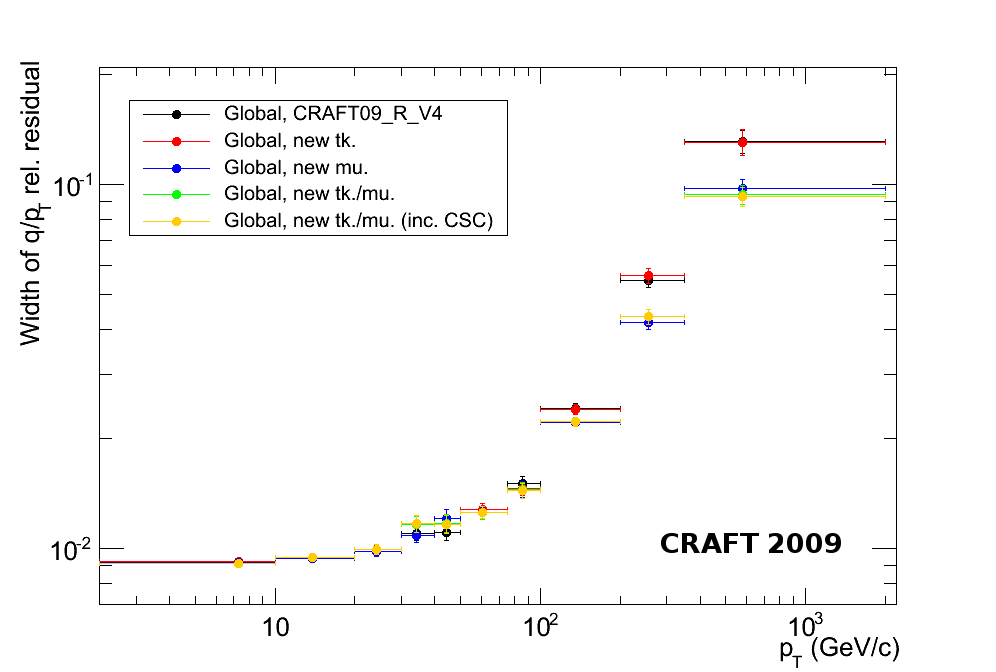
\includegraphics[width=0.5\linewidth]{GlobalMuon.png}

\mbox{ } \hfill {\scriptsize \textcolor{darkblue}{J.~Tucker}}

\vfill
\begin{itemize}
\item DT alignment yields improvements in standAloneMuons (left), globalMuons (right), and FirstMuonStation (not shown)
\item All reconstructions with new CRAFT-09 muon geometry (blue,
  green, yellow) are significantly lower (better) than all
  reconstructions with old CRAFT-08 muon geometry (red and black)
\item GlobalMuon $p_T$ resolution at 200~GeV: 4.2\%
\item FirstMuonStation $p_T$ resolution at 200~GeV: 4.0\%
\end{itemize}
\end{frame}

\begin{frame}
\frametitle{CSC alignment}

\begin{columns}
\column{0.7\linewidth}
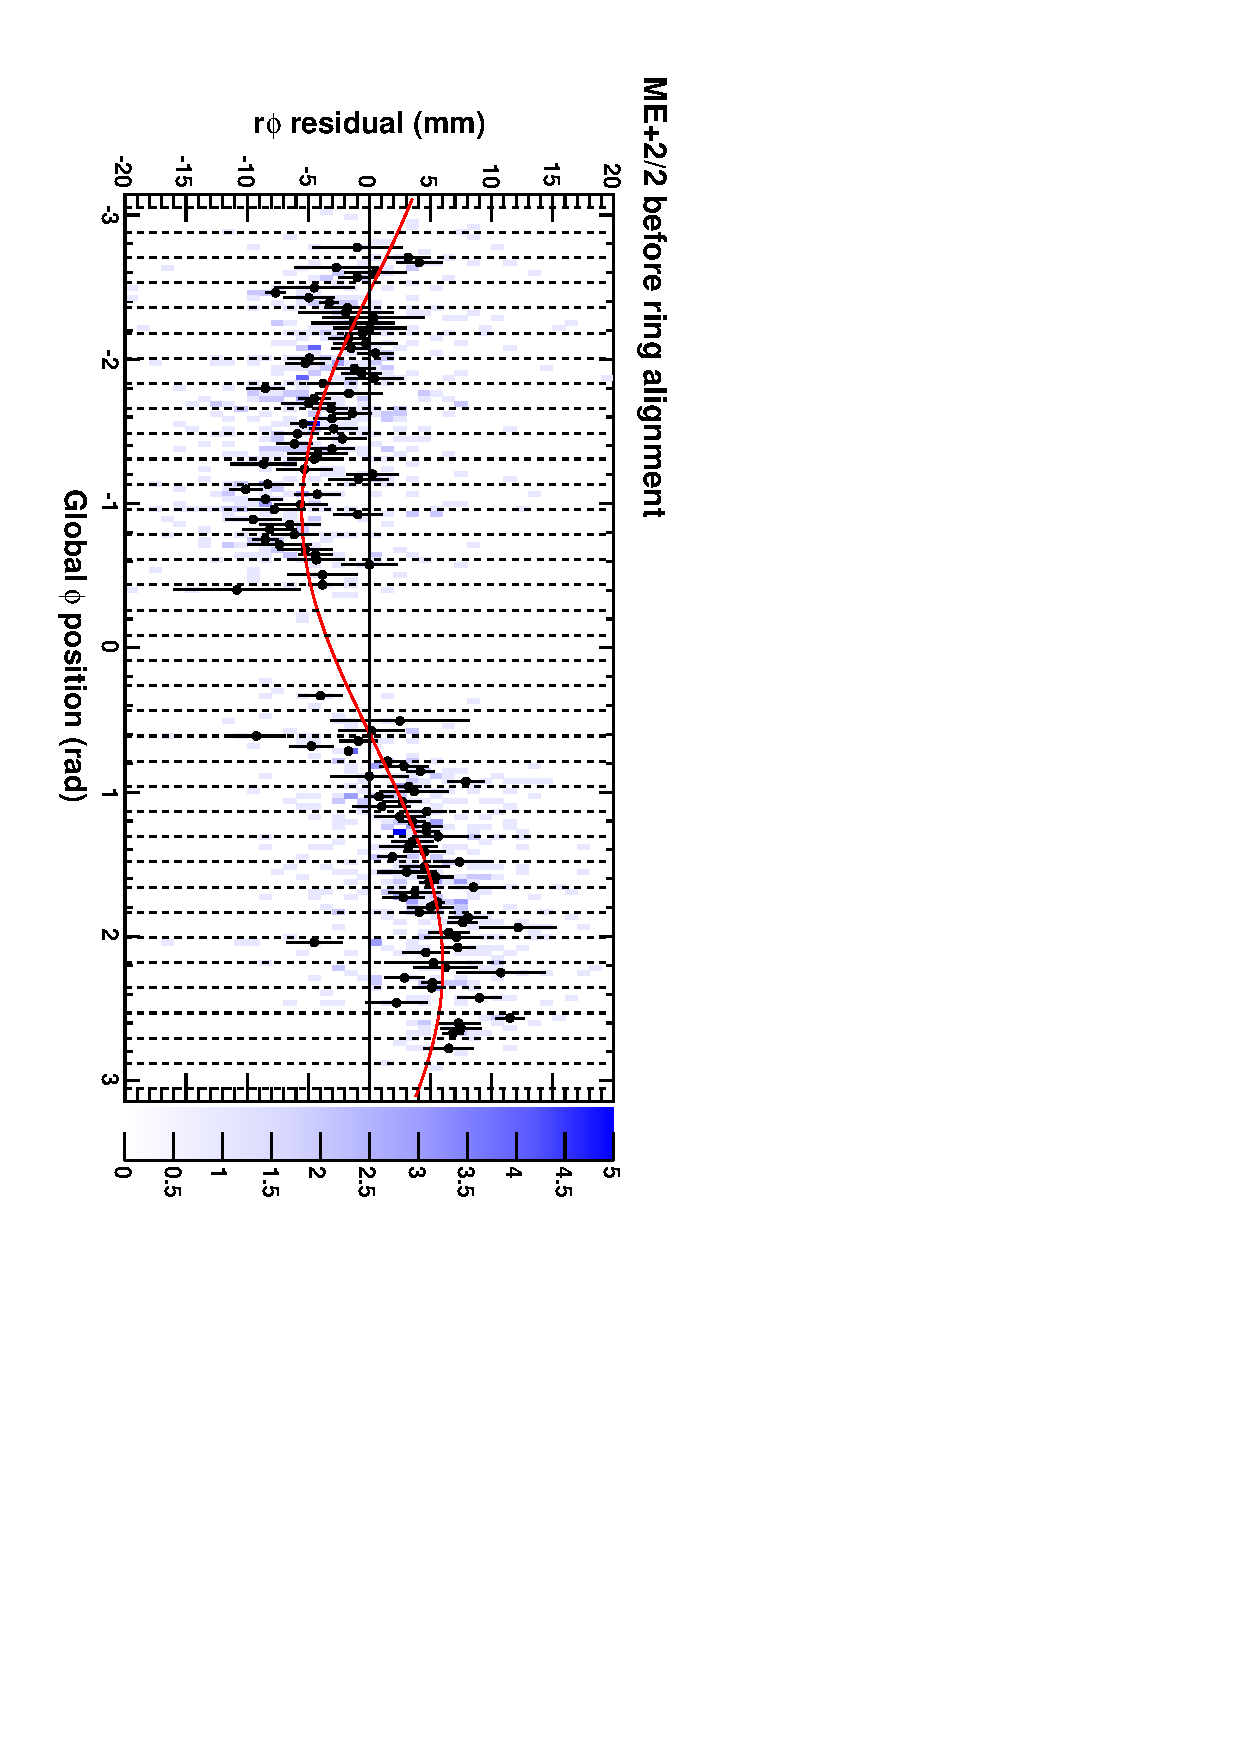
\includegraphics[height=\linewidth, angle=90]{NOV4_ringfits_before/mep22.pdf}

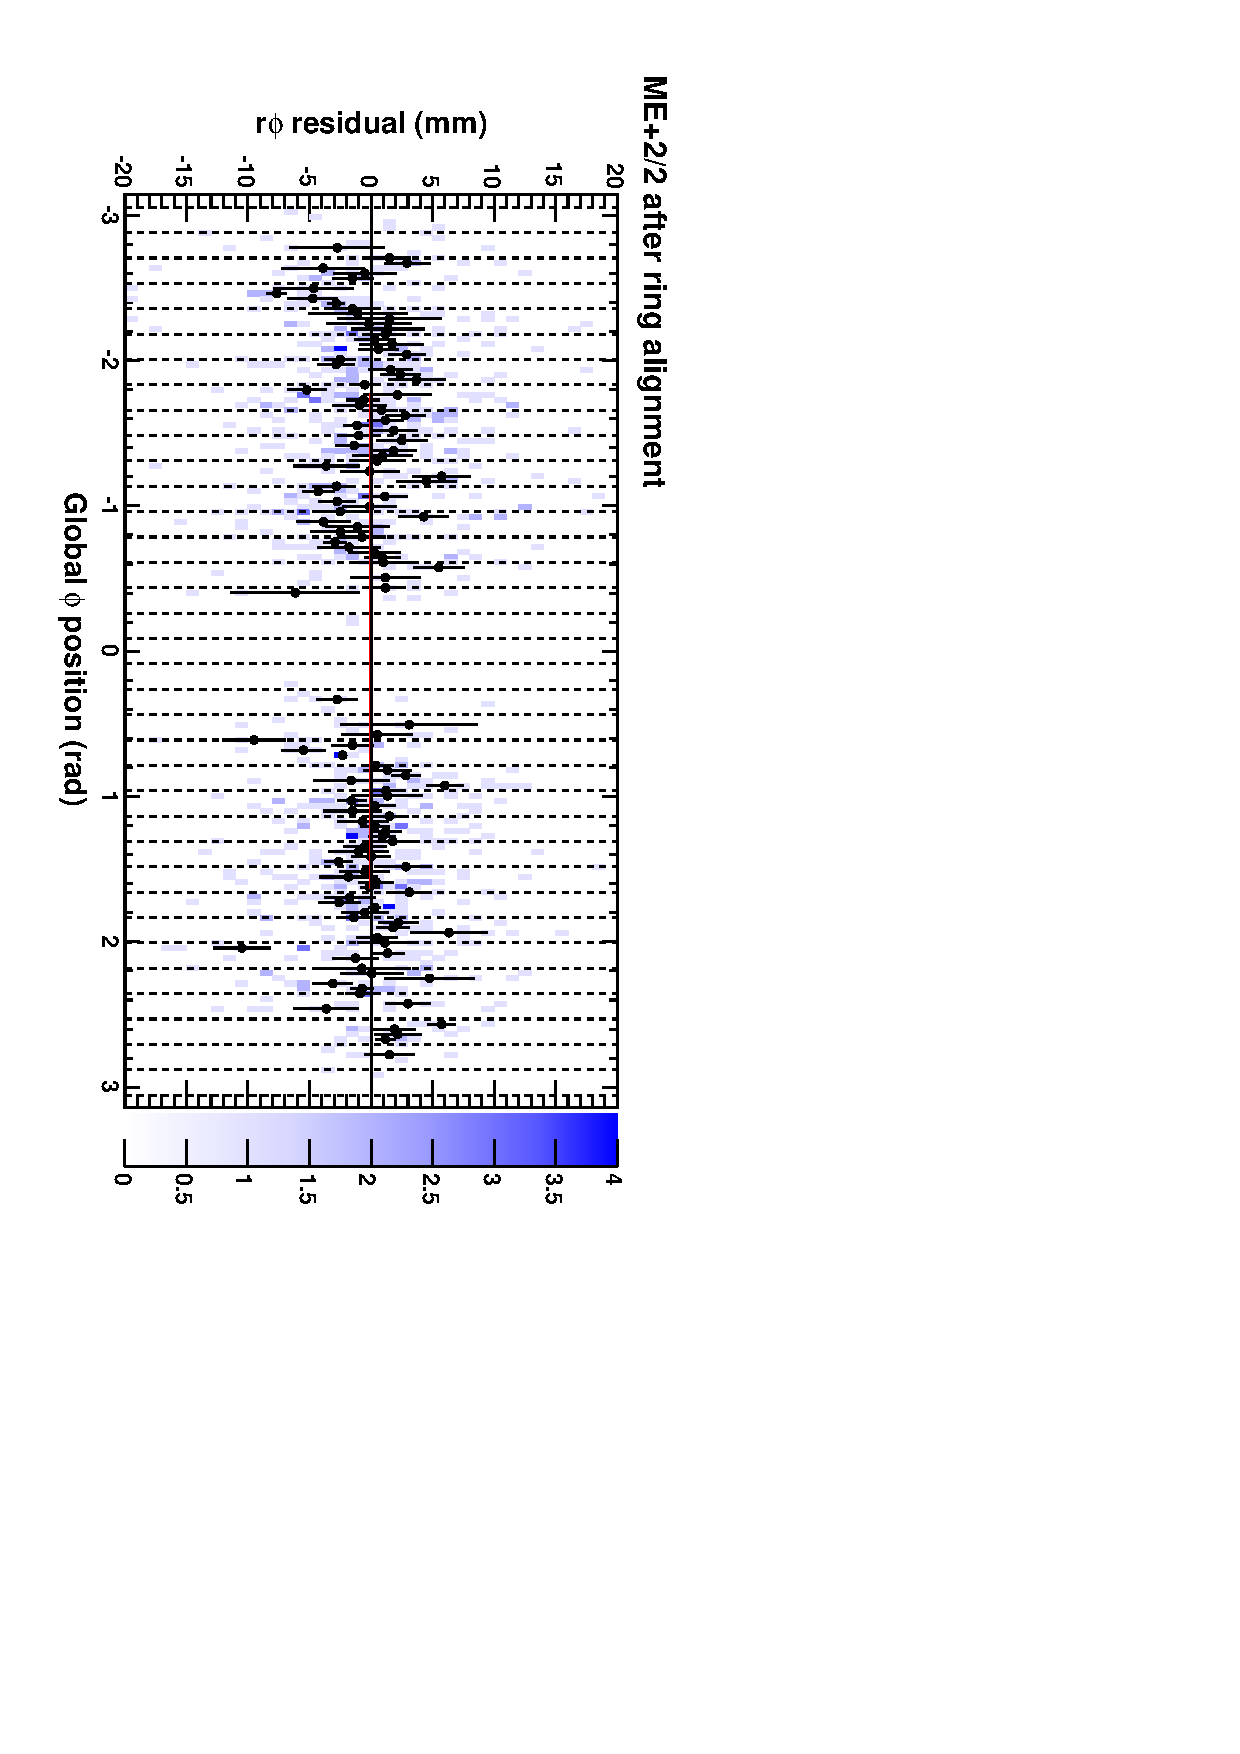
\includegraphics[height=\linewidth, angle=90]{NOV4_ringfits_after/mep22.pdf}

\column{0.3\linewidth}
\begin{itemize}
\item Not enough tracks to align individual chambers
\item Global ring offsets can be inferred from sinusoidal distribution of residuals
\item Large corrections correlated by disk, as expected from closing
\end{itemize}
\end{columns}
\end{frame}

\begin{frame}
\frametitle{Concluding remarks}
\begin{itemize}\setlength{\itemsep}{0.5 cm}
\item Milestone: barrel hardware geometry completely reconstructed, delivered to CMSSW
\item Well-defined procedure agreed upon and implemented
\item Track-based results are consistent with the tracker geometry presented in the previous talk
\item Final muon geometries:

\vspace{0.5 cm}
DTAlignmentRcd and DTAlignmentErrorRcd

\mbox{\hspace{-1.25 cm} \tiny \tt /afs/cern.ch/user/p/pivarski/public/DTAlignmentRcd\_CRAFT09\_segments-hardware-globalMuons\_3XY\_v8\_offline.db}

CSCAlignmentRcd

\mbox{\hspace{-1.25 cm} \tiny \tt /afs/cern.ch/user/p/pivarski/public/CSCAlignmentRcd\_CRAFT09\_hardware-globalMuons\_3XY\_v4\_offline.db}

\end{itemize}
\label{numpages}
\end{frame}

\end{document}
